\chapter{生物无机化学}\label{ch:b3:bioinorganic}

我们的血液因含铁而呈红色；鲎的血液在体内无色，
遇空气则变蓝，因为它以铜携带氧。生命利用少数金属离子
完成有机基团无法胜任的工作：可逆地结合氧、
传递单个电子、裂解水、还原氮，使水分子的酸性
强到足以进攻二氧化碳。本章用配位化学的工具分析这些工作：
\omterm{def:b3:bioinorganic:hsab}{硬酸}与\omterm{def:b3:bioinorganic:hsab}{软酸}、
配体场与自旋态、平衡与速率方程，并以
用作药物的金属作结。

\begin{recall}
本科二年级分册讨论了 $\alpha$-氨基酸、侧链与肽、碱基
与核苷酸、配合物、配体场、高自旋与低自旋，以及
硬、软亲核试剂与亲电试剂；本科一年级分册讨论了
络合常数与 pL 标度。\Cref{ch:b3:complex-spectra-magnetism}和
\cref{ch:b3:complex-mechanisms}给出了光谱、马库斯理论以及顺铂的
水合取代；\cref{ch:b3:complex-kinetics}给出了米氏动力学，并
\cref{ch:b3:advanced-nmr}给出了弛豫时间 $T_1$。
\end{recall}

\begin{omfigure}
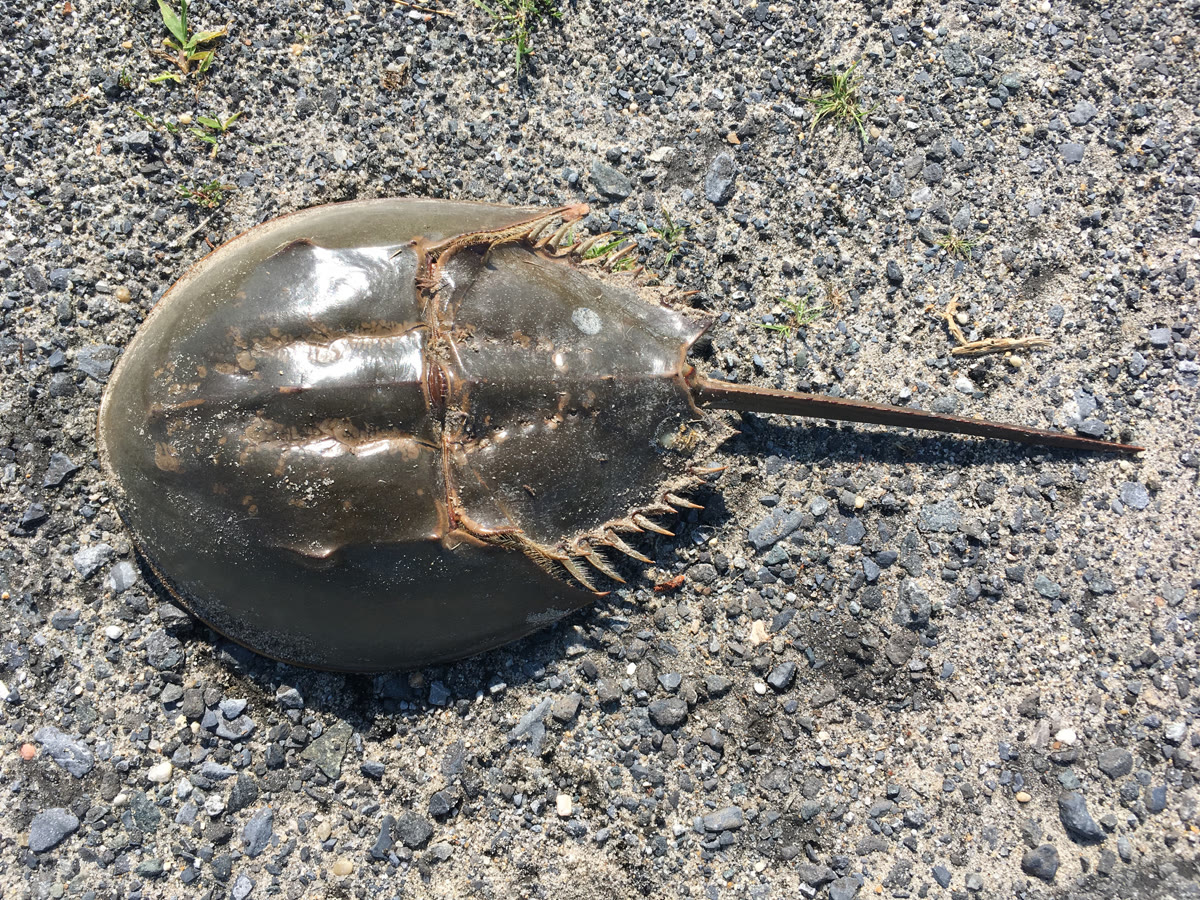
\includegraphics[width=0.5\linewidth]{images/book4/horseshoe-crab.jpg}

{\small 大西洋鲎。其血液以血蓝蛋白携带氧，
血蓝蛋白是一种铜蛋白，氧合后呈蓝色。照片：Kaldari，CC0。}
\end{omfigure}

\section{生物中的金属}

\begin{definition}[金属蛋白]\label{def:b3:bioinorganic:metalloprotein}
称\emph{金属蛋白}\index{金属蛋白}为含有
结合金属离子的蛋白质；\emph{金属酶}\index{金属酶}是能
催化反应的蛋白质。称\emph{辅因子}\index{辅因子}为非蛋白质物种，
即金属离子或小分子，与蛋白质结合，并为其
活性所必需。
\end{definition}

数量上重要的金属是钠、钾、镁和
钙，它们主要带电荷、维持结构；过渡元素
铁、锌、铜、锰、钴、钼和镍含量极少，却主导了大部分化学过程。
蛋白质选择金属，依据的是它所提供的
给体原子及其几何构型。

\begin{definition}[硬酸与软酸]\label{def:b3:bioinorganic:hsab}
称\emph{硬酸}\index{硬酸}为小、高电荷、极化性弱的
路易斯酸（$\ce{H+}$、$\ce{Mg^2+}$、$\ce{Ca^2+}$、$\ce{Fe^3+}$）；称\emph{软
酸}\index{软酸}为大而易极化、低电荷的路易斯酸（$\ce{Cu+}$、$\ce{Ag+}$，
$\ce{Hg^2+}$、$\ce{Cd^2+}$）。\emph{软硬酸碱原理}\index{软硬酸碱原理}
指出：硬酸优先与硬碱结合
（氧给体、氟离子），软酸则与软碱（硫给体、碘离子）结合。
\end{definition}

在蛋白质中，羧酸根与酚盐为硬碱，半胱氨酸的硫醇盐与
蛋氨酸的硫醚为软碱，组氨酸的咪唑介于两者之间。铁(III)
位于氧给体之中，铜(I)位于硫给体之中，锌为
交界酸，与组氨酸和半胱氨酸结合；汞和镉有毒，部分
原因在于它们夺取酶的半胱氨酸。

\begin{definition}[欧文–威廉斯序列]\label{def:b3:bioinorganic:irving-williams}
\emph{欧文–威廉斯序列}\index{欧文–威廉斯序列}是
与给定配体结合时，第一过渡系二价离子的高自旋配合物的
稳定性顺序：
$\ce{Mn^2+} < \ce{Fe^2+} < \ce{Co^2+} < \ce{Ni^2+} < \ce{Cu^2+} > \ce{Zn^2+}$.
\end{definition}

\begin{proposition}[欧文–威廉斯顺序]\label{prop:b3:bioinorganic:irving-williams}
该序列对几乎所有配体都成立（这是一个实验观察结果）；它
遵循从锰到铜离子半径递减的规律、配体场
稳定化能（$d^5$ 时为零，$d^8$ 时最大）以及
铜(II)的姜–泰勒畸变，该畸变使其四个键缩短。
\end{proposition}

\begin{proof}[论证]
同一周期内核电荷增大，半径减小，这增强了
每个配体的静电吸引。高自旋八面体离子的配体场稳定化
能（见\cref{ch:b3:complex-spectra-magnetism}）为 $0$、$4$、
$8$、$12$ 和 $6\,\mathrm{Dq}$，对应 $d^5$ 至 $d^9$；$0$ 对应 $d^{10}$：它直至镍都助长这一趋势，并
在锌处下降；铜(II)借助其四方畸变，
获得超出稳定化能所示的稳定性，该畸变形成四个短而强的键。
\end{proof}

细胞必须应对的一个后果是：铜和锌会胜过
其他离子占据大多数位点，因此其游离浓度被
维持在极低水平，依靠专门的载体蛋白实现。

\section{氧的运输}

\begin{definition}[卟啉与血红素]\label{def:b3:bioinorganic:haem}
称\emph{卟啉}\index{卟啉}为大型平面芳香大环，由四个
吡咯环经次甲基桥连接而成，其四个氮原子与位于中心的一个金属离子结合。
\emph{血红素}\index{血红素}是原卟啉 IX 的铁配合物，
为血红蛋白、肌红蛋白和细胞色素的\omterm{def:b3:bioinorganic:metalloprotein}{辅因子}。
\end{definition}

在肌红蛋白和血红蛋白中，\omterm{def:b3:bioinorganic:haem}{血红素}的铁在环下方有第五个
配体，即近端组氨酸的氮，另有第六个位点可供 $\ce{O2}$ 结合。
脱氧铁(II)为高自旋：一个电子位于 $d_{x^2-y^2}$ 轨道，指向四个
氮原子，对环的\omterm{def:b3:solid-state:carriers}{空穴}而言过大，于是它离开
平面，朝向组氨酸。结合 $\ce{O2}$ 后，它转为低自旋、半径变小，
并移入平面，带动组氨酸和蛋白质螺旋一同移动。

\begin{omfigure}
% ledger: pdb:Hb.deoxy.FeN4, pdb:Hb.oxy.FeN4
\begin{tikzpicture}[font=\small, scale=0.9]
  \foreach \x/\lab/\dz/\oxy in {0/脱氧（高自旋）/-0.34/0, 6.4/氧合（低自旋）/-0.04/1} {
    \begin{scope}[xshift=\x cm]
      \draw[omDef, line width=2.6pt] (-2.2,0) -- (2.2,0);
      \node[font=\scriptsize, anchor=west, omDef] at (2.3,0) {卟啉};
      \fill[omThm] (0,\dz*1.5) circle (0.22);
      \node[font=\scriptsize, anchor=north west] at (0.2,\dz*1.5-0.12) {Fe};
      \draw[black!70, line width=1pt] (0,\dz*1.5-0.22) -- (0,-1.55);
      \node[draw=black!70, regular polygon, regular polygon sides=5, minimum size=7mm, inner sep=0pt] at (0,-1.95) {};
      \node[font=\scriptsize, anchor=west] at (0.45,-1.95) {近端组氨酸};
      \node[font=\small\bfseries] at (0,1.9) {\lab};
      \ifnum\oxy=1
        \draw[black!70, line width=1pt] (0,0.2) -- (0,0.85) -- (0.55,1.25);
        \fill[red!75] (0,0.85) circle (0.13) (0.55,1.25) circle (0.13);
        \node[font=\scriptsize, anchor=west] at (0.75,1.2) {$\ce{O2}$，弯曲};
      \fi
    \end{scope}
  }
  \draw[<->, black!60] (-1.0,0) -- (-1.0,-0.51) node[midway, left, font=\scriptsize] {\qty{0.34}{\angstrom}};
\end{tikzpicture}

{\small 侧视的\omterm{def:b3:bioinorganic:haem}{血红素}铁，其偏离环平面的位移按比例绘制（
1~\AA{} 画作 1.35~cm；其他距离为示意）。脱氧血红蛋白中，高自旋铁（II）
位于四个吡咯氮平均平面之下 \qty{0.34}{\angstrom}，在近端组氨酸一侧；
氧合血红蛋白中，铁位于平面 \qty{0.05}{\angstrom} 以内，$\ce{O2}$
以端基弯曲方式结合（距离由晶体结构计算得出）。}
\end{omfigure}

结合的氧气更宜描述为铁（III）上的超氧化物，$\ce{Fe^{III}-O2^-}$，而非
铁（II）上的中性 $\ce{O2}$：该配合物呈抗磁性，因为两个中心的未成对
电子发生耦合。蛋白质阻止了不可逆的
氧化（生成铁（III）与水），裸露的\omterm{def:b3:bioinorganic:haem}{血红素}在水中会
立即发生这一反应。

\begin{definition}[协同结合]\label{def:b3:bioinorganic:cooperativity}
与具有若干位点的蛋白质的结合，当一个配体的结合
提高了其余位点的亲和力时，称为\emph{协同结合}\index{协同结合}。
\emph{希尔系数}\index{希尔系数} $n$ 为希尔图在半饱和时的斜率，
希尔图即以 $\log\frac{\theta}{1 - \theta}$ 对 $\log p$ 作图，
（$\theta$ 为被占据位点的分数）。
\end{definition}

\begin{proposition}[单个位点]\label{prop:b3:bioinorganic:hyperbola}
对于仅有一个位点的蛋白质，$\mathrm{P + O_2 \rightleftharpoons PO_2}$，占据分数为 $\theta = p/(p_{50} + p)$，其中 $p_{50}$
为以压强表示的解离常数。
\end{proposition}

\begin{proof}
$K_d = [\mathrm P]p/[\mathrm{PO_2}] = p_{50}$，故 $[\mathrm{PO_2}] = [\mathrm P]p/p_{50}$，且 $\theta = [\mathrm{PO_2}]/([\mathrm P] + [\mathrm{PO_2}]) = (p/p_{50})/(1 + p/p_{50})$。
\end{proof}

\begin{theorem}[希尔方程]\label{thm:b3:bioinorganic:hill}
对于具有 $n$ 个位点、且各位点或全空或全占据的蛋白质，
$\mathrm{P + n\,O_2 \rightleftharpoons P(O_2)_n}$,
\[
  \theta = \frac{p^n}{p_{50}^n + p^n}, \qquad \log\frac{\theta}{1 - \theta} = n\log p - n\log p_{50}.
\]
\end{theorem}

\begin{proof}
$K_d = [\mathrm P]p^n/[\mathrm{P(O_2)_n}]$；记 $K_d = p_{50}^n$。被占据位点的分数
即填充形式分子所占的比例，$\theta = [\mathrm{P(O_2)_n}]/([\mathrm P] + [\mathrm{P(O_2)_n}]) = (p/p_{50})^n/(1 + (p/p_{50})^n)$。于是 $\theta/(1 - \theta) = (p/p_{50})^n$，取
对数即得斜率为 $n$ 的直线。
\end{proof}

血红蛋白具有四个位点，但并非完全协同，其\omterm{def:b3:bioinorganic:cooperativity}{希尔系数}
远低于 4，约为 3；其希尔图在两端斜率均为 1，此时它
表现为脱氧或氧合蛋白质，各位点相互独立。协同性源于四级结构
的变化：第一个结合 $\ce{O2}$ 的\omterm{def:b3:bioinorganic:haem}{血红素}中，铁进入平面的运动
被传递给其他亚基。

\begin{omfigure}
\begin{tikzpicture}
\begin{axis}[name=a, width=0.48\linewidth, height=5.6cm, xmin=0, xmax=14, ymin=0, ymax=1.02,
  axis lines=left, xlabel={$p(\ce{O2})$ / \unit{kPa}}, ylabel={饱和度 $\theta$},
  tick label style={font=\scriptsize}, label style={font=\small}]
\addplot[omMeth, thick] table[x=p, y=Mb] {figdata/out/bachelor-3-oxygen-binding.dat};
\addplot[omThm, thick] table[x=p, y=Hb] {figdata/out/bachelor-3-oxygen-binding.dat};
\addplot[omThm, thick, dashed] table[x=p, y=Hbacid] {figdata/out/bachelor-3-oxygen-binding.dat};
\draw[black!35] (axis cs:5,0) -- (axis cs:5,1.0) (axis cs:13,0) -- (axis cs:13,1.0);
\node[font=\scriptsize, anchor=south] at (axis cs:5,0.02) {组织};
\node[font=\scriptsize, anchor=south east] at (axis cs:13,0.02) {肺};
\node[font=\scriptsize, omMeth] at (axis cs:1.9,0.96) {肌红蛋白};
\node[font=\scriptsize, omThm] at (axis cs:7.5,0.6) {血红蛋白};
\end{axis}
\begin{axis}[at={(a.east)}, anchor=west, xshift=1.4cm, width=0.48\linewidth, height=5.6cm,
  xmin=-1.5, xmax=1.5, ymin=-3, ymax=3, axis lines=left,
  xlabel={$\log_{10}(p/\unit{kPa})$}, ylabel={$\log_{10}\bigl(\theta/(1-\theta)\bigr)$},
  tick label style={font=\scriptsize}, label style={font=\small}]
\draw[black!30] (axis cs:-1.5,0) -- (axis cs:1.5,0);
\addplot[omMeth, thick] table[x=lgp, y=Mb] {figdata/out/bachelor-3-oxygen-binding-b.dat};
\addplot[omThm, thick, restrict y to domain=-3:3] table[x=lgp, y=Hb] {figdata/out/bachelor-3-oxygen-binding-b.dat};
\node[font=\scriptsize, omMeth, anchor=west] at (axis cs:-1.1,1.4) {斜率 1};
\node[font=\scriptsize, omThm, anchor=west] at (axis cs:0.75,-1.5) {斜率 2.7};
\end{axis}
\end{tikzpicture}

{\small 左图：肌红蛋白（绿色）与血红蛋白（红色；
虚线：较低 pH 下）的氧饱和度随氧分压的变化，模型取值
$p_{50} = \qty{0.37}{kPa}$（肌红蛋白）与 \qty{3.5}{kPa}（血红蛋白），$n = 2.7$。在肺与组织之间，血红蛋白
释放约四分之一的氧，肌红蛋白几乎不释放。右图：对应的希尔图，
在本模型中为直线（实际血红蛋白的希尔图
在两端弯至斜率 1）。}
\end{omfigure}

\begin{method}[读取希尔图]\label{met:b3:bioinorganic:hill-plot}
\begin{enumerate}
  \item 由每个测得的饱和度计算 $\log(\theta/(1 - \theta))$，并将其对 $\log p$ 作图。
  \item 图线与零线相交处的压强即为 $p_{50}$。
  \item 该点处的斜率即为\omterm{def:b3:bioinorganic:cooperativity}{希尔系数}：$n = 1$ 表示位点相互独立，
        $n > 1$ 表示\omterm{def:b3:bioinorganic:cooperativity}{协同结合}。
  \item 仅有两点时，$n = \Delta\log(\theta/(1 - \theta))/\Delta\log p$。
\end{enumerate}
\end{method}

血红蛋白还在远离\omterm{def:b3:bioinorganic:haem}{血红素}的位点结合质子与二氧化碳，
这些物质在活动组织中含量较高，使其曲线右移：
玻尔效应使氧气恰好在需要之处释放得更多。

\begin{proposition}[一氧化碳竞争]\label{prop:b3:bioinorganic:haldane}
若一氧化碳与氧气竞争同一位点，
反应 $\mathrm{HbO_2 + CO \rightleftharpoons HbCO + O_2}$ 的平衡常数为 $M$，则
$[\mathrm{HbCO}]/[\mathrm{HbO_2}] = M\,p(\ce{CO})/p(\ce{O2})$。
\end{proposition}

\begin{proof}
平衡时 $M = [\mathrm{HbCO}]\,p(\ce{O2})/([\mathrm{HbO_2}]\,p(\ce{CO}))$；整理即得结论。
\end{proof}

$M$ 对人血红蛋白为数百量级，因此只需百万分之数百的一氧化碳
即可占据大部分位点；更糟的是，剩余的空闲位点因协同作用
而更紧密地结合其氧。游离\omterm{def:b3:bioinorganic:haem}{血红素}结合一氧化碳的能力强得多：
在蛋白质中，铁上方的远端组氨酸阻碍一氧化碳偏好的
线性 Fe--C--O 几何构型，同时与弯曲的 $\ce{O2}$ 形成氢键。
其他动物使用其他金属：
软体动物与节肢动物的血蓝蛋白在两个铜离子之间以过氧化物形式结合 $\ce{O2}$，
某些海洋蠕虫的血红蚓蛋白
则在一对铁离子上结合氧。

\begin{inthelab}[氧结合曲线]
将血红蛋白溶于缓冲液，置于配有侧瓶的
气密比色皿中。先通入氮气驱除氧气，然后
注入已知体积的空气，轻轻倾斜比色皿使溶液平衡。
每次加入后记录可见光谱：脱氧型的
谱带（\qty{555}{nm} 附近有一条）让位于氧合型的两条谱带，
并在某一波长处由吸光度读出饱和度，该波长
下的吸光度介于脱氧型与氧合型的极限之间。
\end{inthelab}

\section{金属酶}

碳酸酐酶加快 $\ce{CO2 + H2O <=> HCO3- + H+}$ 的反应，该反应在水中单独进行需要
数秒，这一时间对红细胞短暂流经肺部的
毛细血管足以产生影响。其锌离子由三个组氨酸与一个水分子配位。
作为高电荷的小阳离子，它使该水分子的 $\mathrm pK_a$ 由约 14 降至约 7：
在生理 pH 下，相当一部分酶带有与锌结合的
氢氧根，为强亲核试剂，紧邻一个结合 $\ce{CO2}$ 的口袋。

\begin{omfigure}
\begin{tikzpicture}[font=\small, >=Stealth]
  \node (a) at (90:2.0) {$\mathrm{(His)_3Zn{-}OH_2}$};
  \node (b) at (0:2.9) {$\mathrm{(His)_3Zn{-}OH^-}$};
  \node (c) at (-90:2.0) {$\mathrm{(His)_3Zn{-}OCO_2H^-}$};
  \draw[->, thick] (a) to[bend left=25] node[midway, above right, font=\scriptsize] {$-\,\ce{H+}$（经组氨酸穿梭）} (b);
  \draw[->, thick] (b) to[bend left=25] node[midway, below right, font=\scriptsize, align=left] {$+\,\ce{CO2}$：\\ 亲核进攻} (c);
  \draw[->, thick] (c) to[bend left=35] node[midway, left, font=\scriptsize, align=right] {$+\,\ce{H2O}$\\ $-\,\ce{HCO3-}$} (a);
\end{tikzpicture}

{\small 碳酸酐酶的催化循环。与锌结合的水失去一个
质子；与锌结合的氢氧根进攻二氧化碳；水取代了
碳酸氢根。质子转移至溶剂是最慢的一步。}
\end{omfigure}

\begin{proposition}[快速的酶]\label{prop:b3:bioinorganic:carbonic-anhydrase}
碳酸酐酶的\omterm{def:b3:complex-kinetics:michaelis}{专一性常数} $k_{\mathrm{cat}}/K_M$ 接近于
$\ce{CO2}$ 与该酶的碰撞速率常数：几乎每次碰撞都导致
反应。
\end{proposition}

\begin{proof}[论证]
$k_{\mathrm{cat}}/K_M$ 是底物浓度很低时酶与底物的二级
速率常数（见\cref{ch:b3:complex-kinetics}），它不能超过
二者相遇的扩散控制速率常数
（见\cref{ch:b3:rate-theories}）。碳酸酐酶的实测值
在已知的酶中名列前茅，并接近该极限：\omterm{def:b3:complex-kinetics:enzyme}{活性位点}内部的
化学过程便不再是限制速率的因素。
\end{proof}

细胞色素 P450 酶存在于肝脏及许多其他细胞中，使药物和激素的 C--H
键羟基化。其\omterm{def:b3:bioinorganic:haem}{血红素}中的铁由一个半胱氨酸硫醇盐配位；
$\ce{O2}$ 与两个电子作用，形成\omterm{def:b3:bioinorganic:haem}{卟啉}上带有自由基的铁(IV)-氧代
配合物，称为化合物 I，它从底物夺取一个氢原子，
并将羟基交给碳自由基。固氮酶
在室温下将 $\ce{N2}$ 还原为氨，作用于由七个铁原子
、一个钼和九个硫化物围绕一个中心碳原子构成的 FeMo
\omterm{def:b3:bioinorganic:metalloprotein}{辅因子}，需消耗大量 ATP 分子。维生素 $\mathrm{B_{12}}$ 含有一个
钴–碳键，是生物中极少数金属–碳键之一，其
均裂引发自由基重排。

\section{电子转移与能量}

只负责传递电子的蛋白质，其金属中心的
\omterm{def:b3:complex-mechanisms:reorganisation}{重组能}（见\cref{ch:b3:complex-mechanisms}）较小：两种氧化态的
几何构型几乎相同，因此马库斯势垒较低。

\begin{definition}[铁硫簇]\label{def:b3:bioinorganic:fes}
\emph{铁硫簇}\index{铁硫簇}是一组由硫离子桥连、
并通过半胱氨酸硫醇盐与蛋白质结合的铁离子：
$\ce{[2Fe-2S]}$、$\ce{[3Fe-4S]}$ 和立方烷型的 $\ce{[4Fe-4S]}$。
\end{definition}

\begin{definition}[蓝铜蛋白]\label{def:b3:bioinorganic:blue-copper}
\emph{蓝铜蛋白}\index{蓝铜蛋白}含有一个铜离子，
由两个组氨酸、一个半胱氨酸和一个弱结合的甲硫氨酸配位，位于
畸变的四面体位点中；其强烈的蓝色来源于
半胱氨酸到铜(II)的电荷转移吸收带。
\end{definition}

\begin{definition}[张力态]\label{def:b3:bioinorganic:entatic}
\emph{张力态}\index{张力态}是蛋白质使金属位点保持的一种
应变几何构型，介于其两种氧化态偏好的几何构型之间，
从而降低其反应的\omterm{def:b3:complex-mechanisms:reorganisation}{重组能}。
\end{definition}

铜(II)单独时偏好平面正方形，铜(I)偏好四面体；在蓝铜
位点中两种偏好都不能满足，因此电子转移很快。

\begin{definition}[放氧复合体]\label{def:b3:bioinorganic:oec}
\emph{放氧复合体}\index{放氧复合体}是
光系统~II 中的 $\mathrm{Mn_4CaO_5}$ 簇，在
光合作用中将水氧化为氧气。
\end{definition}

\begin{proposition}[每个氧需四个光子]\label{prop:b3:bioinorganic:kok}
将两个水分子氧化为一个 $\ce{O2}$，需要光系统~II
吸收四个光子，该簇经历五个状态 $\mathrm S_0$ 至 $\mathrm S_4$。
\end{proposition}

\begin{proof}
$\ce{2H2O -> O2 + 4H+ + 4e-}$：必须移去四个电子。被反应中心
吸收的每个光子使一个电子离开，簇则逐个电子地
补充被氧化的中心：四个光子、四步，逐步储存
氧化当量于 $\mathrm S_1$ 至 $\mathrm S_4$ 诸状态中；$\mathrm S_4$ 释放 $\ce{O2}$ 并回到 $\mathrm S_0$。
\end{proof}

\begin{omfigure}
\begin{tikzpicture}[font=\small, >=Stealth]
  \foreach \i/\ang in {0/90, 1/18, 2/-54, 3/-126, 4/162} {
    \node[draw, circle, minimum size=9mm, fill=omDef!10] (s\i) at (\ang:2.0) {$\mathrm S_{\i}$};
  }
  \foreach \i/\j in {0/1, 1/2, 2/3, 3/4} {
    \draw[->, thick] (s\i) to[bend left=18] node[midway, sloped, above, font=\scriptsize] {$h\nu$, $-\mathrm e^-$} (s\j);
  }
  \draw[->, thick, omThm] (s4) to[bend left=18] node[midway, sloped, above, font=\scriptsize] {$-\ce{O2}$, $+\,\ce{2H2O}$} (s0);
\end{tikzpicture}

{\small \omterm{def:b3:bioinorganic:oec}{放氧复合体}的科克循环。每个被
光系统~II 吸收的光子从锰簇中移去一个电子（途中有质子
离开）；第四次氧化给出 $\mathrm S_4$，它释放双原子氧，
并重新结合两个水分子。}
\end{omfigure}

能量链的另一端，线粒体中的细胞色素 $c$ 氧化酶
用四个电子和四个质子把 $\ce{O2}$ 还原为水，反应
在彼此相对的一个\omterm{def:b3:bioinorganic:haem}{血红素}铁与一个铜离子上进行，
且不释放出部分还原、有害的超氧化物或过氧化物。

\section{金属在医学中的应用}

\begin{definition}[金属药物]\label{def:b3:bioinorganic:metallodrug}
称\emph{金属药物}\index{金属药物}为一种活性依赖于
金属离子或金属配合物的药物。
\end{definition}

顺铂 \textit{cis}-$\ce{[PtCl2(NH3)2]}$ 在血液中稳定，此处氯离子浓度
高；在细胞内，氯离子浓度低得多，它与水交换一个氯离子
（见\cref{ch:b3:complex-mechanisms}）。水合配合物与鸟嘌呤的 N7 原子
结合，随后同链上紧邻的第二个鸟嘌呤也结合：1,2-GG
交联使 DNA 弯曲，细胞无法修复，于是死亡。
\textit{trans} 同分异构体不能桥连两个相邻碱基，因而无活性。
卡铂带有一个螯合的二羧酸根，离去缓慢，
副作用较少；奥沙利铂带有二氨基环己烷配体，
对顺铂耐药的肿瘤仍然有效。

\begin{omfigure}
\begin{tikzpicture}[font=\small]
  \draw[black!60, line width=1.4pt] (-3.2,0) -- (3.2,0);
  \node[font=\scriptsize, anchor=west] at (3.3,0) {DNA 链};
  \foreach \x/\b in {-2.4/C, -1.0/G, 1.0/G, 2.4/T} {
    \draw[black!60, line width=1pt] (\x,0) -- (\x,0.6);
    \node[draw=black!70, fill=white, rounded corners=1pt, minimum width=6mm] (n\b\x) at (\x,0.9) {\b};
  }
  \node (pt) at (0,2.4) {$\ce{Pt}$};
  \draw[omThm, thick] (pt) -- (-0.95,1.2) node[midway, left, font=\scriptsize] {N7};
  \draw[omThm, thick] (pt) -- (0.95,1.2) node[midway, right, font=\scriptsize] {N7};
  \draw (pt) -- (-0.5,3.1) node[above left, font=\scriptsize, inner sep=1pt] {$\ce{H3N}$};
  \draw (pt) -- (0.5,3.1) node[above right, font=\scriptsize, inner sep=1pt] {$\ce{NH3}$};
\end{tikzpicture}

{\small 顺铂形成的 1,2-链内交联示意：失去
两个氯离子后，铂与同一链上相邻两个鸟嘌呤的 N7
原子结合，并保留两个 \textit{cis} 氨配体。真实的加合物
会使双螺旋弯曲。}
\end{omfigure}

\begin{definition}[造影剂]\label{def:b3:bioinorganic:contrast}
用于磁共振成像的\emph{造影剂}\index{造影剂}是一种
能缩短附近水分子质子弛豫时间的顺磁性化合物。
其\emph{弛豫率}\index{弛豫率} $r_1$ 为
单位造影剂浓度下弛豫速率 $1/T_1$ 的增量。
\end{definition}

\begin{proposition}[弛豫速率]\label{prop:b3:bioinorganic:relaxivity}
设\omterm{def:b3:bioinorganic:contrast}{造影剂}\omterm{def:b3:bioinorganic:contrast}{弛豫率}为 $r_1$、浓度为 $c$，则水质子的
弛豫速率为 $1/T_1 = 1/T_{1,0} + r_1c$，其中 $T_{1,0}$ 为无\omterm{def:b3:bioinorganic:contrast}{造影剂}时的值。
\end{proposition}

\begin{proof}
顺磁贡献正比于单位时间内水分子所访问的
\omterm{def:b3:bioinorganic:contrast}{造影剂}分子数，因而正比于 $c$；独立机制产生的弛豫速率
可以相加。由 $r_1$ 的定义，附加速率为 $r_1c$。
\end{proof}

钆（III），$4f^7$，具有七个未成对电子和弛豫缓慢的
电子自旋，是首选金属。游离的 $\ce{Gd^3+}$ 有毒，因此它
以极稳定的八齿多氨基羧酸根配合物形式给药，该配合物只留出一个
位点给一个水分子，该水分子与本体溶液快速交换，并将
弛豫效应传递到整个本体溶液。

\begin{definition}[螯合疗法]\label{def:b3:bioinorganic:chelation-therapy}
\emph{螯合疗法}\index{螯合疗法}是指借助以药物形式给予的螯合配体，将体内的有毒
金属移出体外，该配体与金属形成稳定、可溶的配合物，
随后被排出。
\end{definition}

\begin{method}[选择螯合药物]\label{met:b3:bioinorganic:choose-chelator}
\begin{enumerate}
  \item 比较螯合剂与有毒金属的稳定常数，
        以及它与体内大量存在的必需金属（$\ce{Ca^2+}$、$\ce{Mg^2+}$、
        $\ce{Zn^2+}$）的稳定常数。
  \item 计算螯合剂所留下的游离金属水平 $\mathrm{pM} = -\log[\mathrm M]$，
        即在体内浓度和 pH 下：有毒金属的 pM 越高越好，
        必需金属的 pM 越低越好。
  \item 给药时螯合剂应已载有相互竞争的必需离子（
        即用于铅中毒的 EDTA 钙配合物），使其交换而非
        从血液中夺取钙。
  \item 检查软硬匹配（汞、铅用硫供体，
        铁（III）用硬氧供体），并确认配合物可被排出。
\end{enumerate}
\end{method}

\begin{safety}{\ghs[0.62cm]{GHS05}\ghs[0.62cm]{GHS06}\ghs[0.62cm]{GHS08}}
% ledger: ghs4:cisplatin
顺铂：吞食致命，可能致癌并引起遗传缺陷，可能损害
生育能力，会严重损伤眼睛并引起过敏反应；只能以
已配制的药物溶液形式操作，须戴手套，并在通风橱中进行。
\end{safety}

\begin{history}[一种蛋白质结构与一种偶然发现的药物]
马克斯·佩鲁茨研究血红蛋白的 X 射线结构长达二十多年，
该结构于 1959 年以低分辨率解出；他与解出肌红蛋白结构的约翰·肯德鲁
共同获得了 1962 年诺贝尔化学奖。1965 年，巴尼特·罗森伯格
在细菌培养液中让电流经过铂电极，
他看到细菌长成长丝而不分裂，原因
并非电流，而是电极形成的一种铂氨配合物。它
后来成为顺铂，至今仍是最常用的抗癌药物之一。
\end{history}

\section{练习}

\begin{exercise}[$\star$]\label{exo:b3:bioinorganic:1}
某蛋白质在 \qty{2.1}{kPa} 氧压下饱和度为 20\,\%，在 \qty{5.9}{kPa} 下为 80\,\%。求其
\omterm{def:b3:bioinorganic:cooperativity}{希尔系数}。
\end{exercise}

\begin{exercise}[$\star$]\label{exo:b3:bioinorganic:2}
将 $\ce{Zn^2+}$、$\ce{Mn^2+}$、$\ce{Cu^2+}$、$\ce{Fe^2+}$、$\ce{Ni^2+}$ 和 $\ce{Co^2+}$ 按其与某给定配体形成的配合物的稳定性排序，
并说明锌所处的位置。
\end{exercise}

\begin{exercise}[$\star$]\label{exo:b3:bioinorganic:3}
预测下列离子偏好的蛋白质配位原子（羧酸根、半胱氨酸硫醇根、
组氨酸咪唑）：$\ce{Ca^2+}$、$\ce{Fe^3+}$、$\ce{Cu+}$、$\ce{Zn^2+}$ 和 $\ce{Hg^2+}$。
\end{exercise}

\begin{exercise}[$\star$]\label{exo:b3:bioinorganic:4}
光系统~II 移去的电子数与吸收的光子数各为多少，
以每放出一个 $\ce{O2}$ 分子计？以每摩尔计？
\end{exercise}

\begin{exercise}[$\star\star$]\label{exo:b3:bioinorganic:5}
利用本章的模型曲线（肌红蛋白 $p_{50} = \qty{0.37}{kPa}$；血红蛋白 \qty{3.5}{kPa}，$n = 2.7$），
计算两种蛋白质各自在
\qty{13}{kPa}（肺）与 \qty{5}{kPa}（组织）之间释放出的氧所占的分数。
\end{exercise}

\begin{exercise}[$\star\star$]\label{exo:b3:bioinorganic:6}
吸入含一氧化碳 \qty{50}{ppm} 的空气，时间足够长，直至
达到平衡。取 $M = 230$（题中数据），且 $p(\ce{O2})/p(\ce{CO})$ 取空气中的比值
（含氧 20.95\,\%），求血红蛋白中结合一氧化碳的比例为多少？
\end{exercise}

\begin{exercise}[$\star\star$]\label{exo:b3:bioinorganic:7}
给出下列簇中铁离子的形式氧化态：$\ce{[Fe2S2(SR)4]^2-}$、
$\ce{[Fe2S2(SR)4]^3-}$ 与 $\ce{[Fe4S4(SR)4]^2-}$（SR：半胱氨酸根，S：硫化物）。
\end{exercise}

\begin{exercise}[$\star\star$]\label{exo:b3:bioinorganic:8}
写出顺铂的第一步水合反应，并说明其在血液中为何较慢、
在细胞内却较快。铂与 DNA 的哪个原子结合，
以及 \textit{trans} 异构体为何无活性？
\end{exercise}

\begin{exercise}[$\star\star$]\label{exo:b3:bioinorganic:9}
某组织的 $T_1 = \qty{1.2}{s}$。一种\omterm{def:b3:bioinorganic:contrast}{弛豫率}为 $\qty{4.0}{L.mmol^{-1}.s^{-1}}$ 的钆\omterm{def:b3:bioinorganic:contrast}{造影剂}，
使其中浓度达到 \qty{0.10}{mmol/L}（题中数据）。求新的 $T_1$。
\end{exercise}

\begin{exercise}[$\star\star\star$]\label{exo:b3:bioinorganic:10}
螯合剂 L 的 $\log K = 18.0$ 对应 $\ce{Pb^2+}$，$10.7$ 对应 $\ce{Ca^2+}$（题中数据）。
求反应 $\ce{Pb^2+ + [CaL]^2- <=> [PbL]^2- + Ca^2+}$ 的平衡常数，并说明为何
题中给出的是钙配合物而非游离配体。
\end{exercise}

\begin{exercise}[$\star\star\star$]\label{exo:b3:bioinorganic:11}
% ledger: enz:median.kcatKM
碳酸酐酶的 $k_{\mathrm{cat}}/K_M \approx \qty{1e8}{L.mol^{-1}.s^{-1}}$（题中数据），一种典型酶约为
$\qty{1e5}{L.mol^{-1}.s^{-1}}$。在 $[\ce{CO2}] = \qty{1.0}{mmol/L}$（远低于 $K_M$）时，比较二者各自转化一半底物
所需的时间，酶浓度为 \qty{1.0}{\micro mol/L}。
\end{exercise}

\begin{exercise}[$\star\star\star$]\label{exo:b3:bioinorganic:12}
取 $M = 230$，一氧化碳的压强为多少时可占据一半的
结合位点？空气中氧分压为 \qty{0.2095}{bar}，以 \qty{1}{bar} 下气体的 ppm 数表示。
\end{exercise}

\section{问题：血液能输送多少氧？}

\begin{problem}[{周末问题——血液能输送多少氧？血红蛋白与肌红蛋白的
希尔曲线，一升血液携带的氧，
玻尔效应，以及一氧化碳夺走的部分}]
\label{pb:b3:bioinorganic:1}
% ledger: const:Vm1
题中模型数据：血红蛋白在 pH 7.4 时 $p_{50} = \qty{3.5}{kPa}$ 且 $n = 2.7$，
在工作组织较低的 pH 下 $p_{50} = \qty{4.0}{kPa}$；肌红蛋白 $p_{50} = \qty{0.37}{kPa}$；血液中血红蛋白含量为 \qty{150}{g/L}，
摩尔质量为 \qty{64.5}{kg/mol}，每分子含四个结合位点；$p(\ce{O2})$ 在肺中为 \qty{13}{kPa}，
在组织中为 \qty{5.0}{kPa}；静息时心脏每分钟泵出血液 \qty{5.0}{L/min}；
一氧化碳的 $M = 230$。气体体积均取 \qty{273.15}{K} 与 \qty{101.325}{kPa} 下的值。

\medskip\noindent\textbf{第一部分——曲线。}
\begin{enumerate}
  \item 求血红蛋白在肺中的饱和度。
  \item 求 pH 7.4 时血红蛋白在组织中的饱和度。
  \item 求 \qty{5.0}{kPa} 时肌红蛋白的饱和度。
  \item 为什么肌肉中的肌红蛋白能从血红蛋白中夺取氧？
  \item 若为四个独立位点，\omterm{def:b3:bioinorganic:cooperativity}{希尔系数}应为多少？
  \item 用一句话解释协同性的来源。
\end{enumerate}

\medskip\noindent\textbf{第二部分——一升血液。}
\begin{enumerate}[resume]
  \item 求血红蛋白的浓度，单位为 mol/L。
  \item 求氧结合位点的浓度。
  \item 求肺中每升血液携带的氧，以 mmol 计。
  \item 求 pH 7.4 时每升血液输送到组织的氧。
  \item 将其换算为毫升气体。
  \item 该部分占所携带氧的分数是多少？
\end{enumerate}

\medskip\noindent\textbf{第三部分——玻尔效应。}
\begin{enumerate}[resume]
  \item 求较低 pH 下组织中的饱和度。
  \item 求考虑玻尔效应后每升血液输送的氧。
  \item 该效应使输送量增加到原来的多少倍？
  \item 什么会降低工作肌肉的 pH？
  \item 求静息时每分钟输送的氧，以 mmol 计。
  \item 将其换算为每分钟的气体升数。
\end{enumerate}

\medskip\noindent\textbf{第四部分——一氧化碳。}
\begin{enumerate}[resume]
  \item 求 $[\mathrm{HbCO}]/[\mathrm{HbO_2}]$，取含 \qty{100}{ppm} 一氧化碳的空气。
  \item 求因一氧化碳而失去的结合位点所占的分数。
  \item 为什么输送的氧损失比该分数更严重？
  \item 为什么首选纯氧作为治疗？
  \item 为什么远端组氨酸对生存至关重要？
  \item 给出结论：静息时每分钟输送的氧升数。
\end{enumerate}
\end{problem}
